\textbf{Obtener toda la información de los clientes que viven en Seatle o en San Francisco, que pertenezcan al segmento
corporate que hayan solicitado una orden en el segundo trimestre de 2014. Mostrar la información ordenada por la
cantidad solicitada.} \vspace{.3cm}

La verdad es que la sintaxis de la pregunta deja poco claro lo que se necesita pero yo lo interprete de la siguiente manera:

\begin{center}
    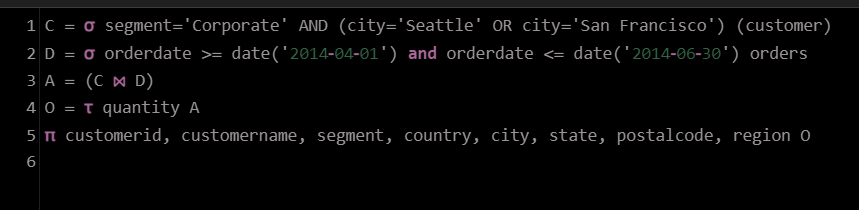
\includegraphics[width=14cm]{resources/pregunta2/2.1.1.png}
\end{center}

La idea es la siguiente, comenzamos por seleccionar a los clientes que viven en Seatle o en San Francisco, que pertenezcan al segmento corporate, eso es una mini consulta. Luego seleccionamos las ordenes que se hicieron en el segundo trimestre de 2014, eso es otra mini consulta. Luego unimos ambas consultas, finalmente ordenamos por la cantidad solicitada, aqui es donde no estoy seguro de si ahi acaba nuestra consulta o, como dice que solo quiere la información de los clientes tenemos que solo regresarle las columnas relevantes (si no hacemos el siguiente paso se van a repetir clientes porque tienen varios pedidos, igual otra opcion es agrupar por cliente), entonces decidi incluir esta ultima aunque si no es necesario podriamos parar ahi, entonces solo proyectamos sobre las columnas de costumer sobre la consulta anterior.

Esto nos regresa la siguiente tabla:

\begin{center}
    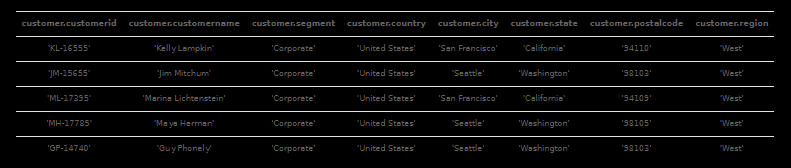
\includegraphics[width=14cm]{resources/pregunta2/2.1.2.png}
\end{center}

Como se ve esto regresa toda la información de los clientes en la forma que se solicita con el detalle de no incluir detalle de la orden.

\newpage